%# -*- coding: utf-8-unix -*-
%%==================================================
%% chapter1.tex for SJTU Master Thesis
%%==================================================

\chapter{基于农业物联网的智能温室架构}
\label{chapter:IoT Architecture}

\section{系统整体架构设计}
	\subsection{物联网层次定义}
	根据一般的物联网架构层次定义\supercite{Yu2011Research,LiuQiang2010},物联网可分为感知层、网络层和应用层三层结构\supercite{HanYi2016A,WangHuaiyu2015},如\ref{fig:ArchitectureIoT}所示。
	\begin{figure}[!htp]
  		\centering
 		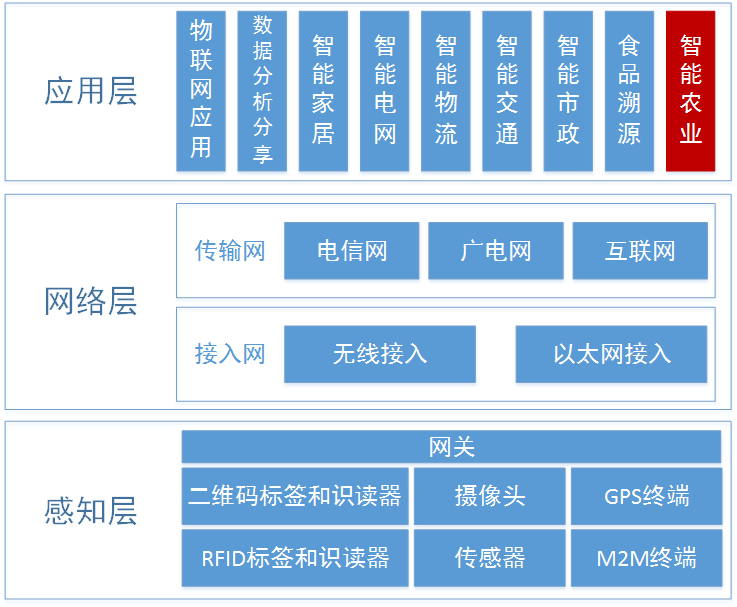
\includegraphics[width=0.8\textwidth]{chapter1/ArchitectureIoT.png}
  		\bicaption[fig:ArchitectureIoT]{物联网层次架构}{物联网层次架构}{Fig}{Architecture of the Internet of Things}
	\end{figure}
	感知层是物联网的核心部分,位于物联网三层结构的最底层,是信息采集的关键部分,是架设在人类世界和物理世界之间的桥梁,主要负责物联网系统的“感知”,相当于人类五官的功能,包含各种感应器件和感应器组成的网络两部分,可以对物体的各类属性和环境状态等数据信息进行动态感知、快速识别和信息采集。该层的核心技术包括射频技术、新兴传感技术、无线网络组网技术、现场总线控制技术等,涉及的核心产品包括二维码标签和识读器、RFID标签和读写器、摄像头、GPS终端、传感器、M2M终端、各类网关等。
	
	网络层是物联网的枢纽部分,位于物联网三层结构中的第二层,是信息传输的重要部分,其功能为“传送”,即通过通信网络进行信息传输。网络层作为纽带连接着感知层和应用层,它由各种私有网络、互联网、有线和无线通信网等组成,相当于人的神经中枢系统,负责将感知层获取的信息,安全可靠地传输到应用层,然后根据不同的应用需求进行信息处理。网络层包含接入网和传输网,分别实现接入功能和传输功能。传输网由公网与专网组成,典型传输网络包括电信网、广电网、互联网等;接入网包括无线接入、以太网接入等各类接入方式,实现底层的传感器网络、RFID网络的接入。物联网的网络层基本上综合了已有的全部网络形式,来构建更加广泛的“互联”。
	
	应用层位于物联网三层结构中的最顶层,主要负责处理各种信息处理。应用层与最低层的感知层一起,是物联网的显著特征和核心所在,应用层可以对感知层采集数据进行计算、处理和知识挖掘,从而实现对物理世界的实时控制、精确管理和科学决策。目前,其核心功能主要围绕数据的管理与处理,以及数据与各行业应用相结合。从结构上划分,物联网应用层主要包括物联网中间件、物联网应用和云计算。从物联网三层结构的发展来看,网络层已经非常成熟,感知层的发展也非常迅速,而应用层不管是从受到的重视程度还是实现的技术成果上,以前都落后于其他两个层面。但因为应用层可以为用户提供具体服务,是与我们最紧密相关的,因此应用层的未来发展潜力很大。
	
	\subsection{智能温室整体架构设计}
	根据一般物联网架构层次定义和农业生产的特殊需求,本文基于农业物联网的智能温室系统自底向上划分为感知控制层、网络传输层和应用层,另外为了兼容各类终端设备接入添加了终端接入层\supercite{WangHuaiyu2015},如\ref{fig:System}所示。
		\begin{figure}[!htp]
  			\centering
 			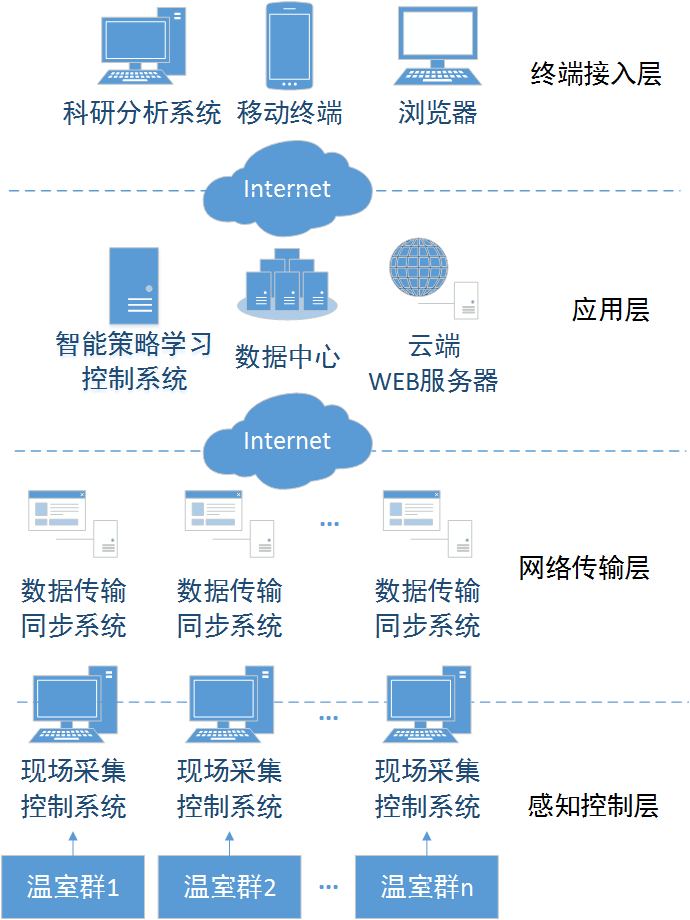
\includegraphics[width=0.6\textwidth]{chapter1/ArchitectureSystem.png}
  			\bicaption[fig:System]{智能温室系统整体架构}{智能温室系统整体架构}{Fig}{Architecture of the intelligent greenhouse system.}
		\end{figure}
		
\section{感知控制层}
感知控制层主要用于获取需要监测及用于控制的各类温室环境参数数据,已经对温室现场的作动器进行控制以达到控制温室内环境参数的目的。本层通过现场采集控制系统实现,其总体设计如\ref{fig:Sensing}所示。针对农业特殊的生产环境,本层适合使用可靠性高、稳定性强、灵活性大、易于扩展的传感器网络采集温室环境参数数据,如基于RS485总线的传感器网络、基于ZigBee的无线传感器网络等。
		\begin{figure}[!htp]
  			\centering
 			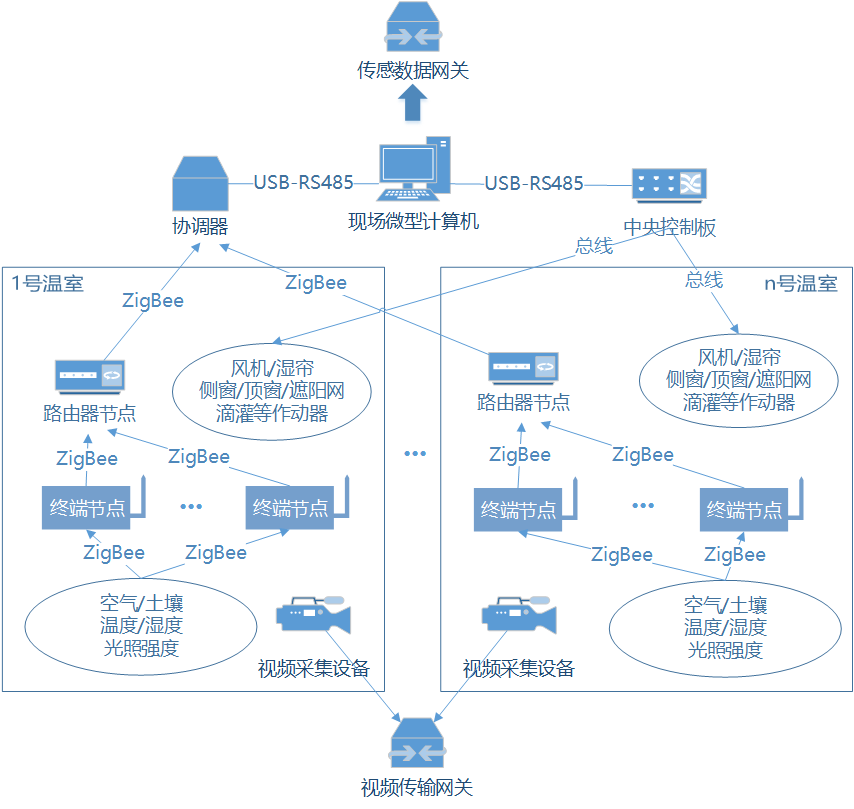
\includegraphics[width=0.8\textwidth]{chapter1/sensing.png}
  			\bicaption[fig:Sensing]{智能温室系统整体架构}{智能温室系统整体架构}{Fig}{Architecture of the intelligent greenhouse system.}
		\end{figure}

监测到当前温室环境后,系统需要通过控制温室内作动器的动作对温室内的环境加以控制,从而达到让温室环境更加适宜温室内作物生长的目的。因此本层还包括用于控制温室内作动器的中央控制板。为降低成本的同时提高设备的可靠性,本系统适合采用嵌入式计算机提供现场计算服务,同时兼用作网关服务,如基于ARM的微型计算机等。另外,为了增加对温室内环境的直观感知,本层添加了图像采集模块,包括图像采集设备和图像传输网关,该模块可在需要视频或图像监测的温室内使用。
\section{网络传输层}

\section{应用层}

\section{终端接入层}
 
